\setAuthor{}
\setRound{piirkonnavoor}
\setYear{2020}
\setNumber{G 3}
\setDifficulty{3}
\setTopic{TODO}

\prob{Hüppav silinder}
\begin{wrapfigure}[10]{r}{0.3\textwidth}
    \vspace{-30pt}
	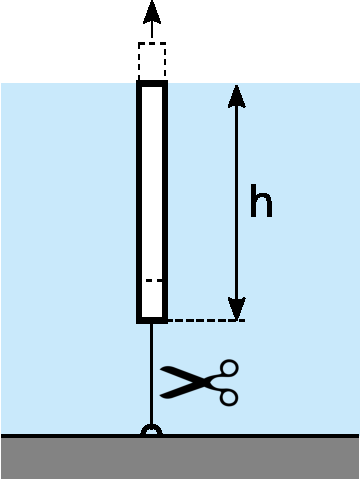
\includegraphics[width=0.3\textwidth]{2020-v2g-03-yl.pdf}
\end{wrapfigure}


Peenike seest tühi silinder on nööriga kinnitatud veega täidetud basseini põhja nii, nagu näidatud joonisel. 
Silindri ülemine ots asub veepinnal. Nöör lõigatakse läbi ja silinder hakkab ülespoole liikuma ning hüppab veest välja. Kui kõrgele õhku tõuseb silindri alumine ots veepinnast maksimaalselt? Eeldage, et veest täielikult väljumise hetkel läheb 50\% silindri kineetilisest energiast kaduma silindri ja veepinna vastastikmõju tõttu. Muude keskkonna takistusjõududega ei pea arvestama.
Silindri mass $m = \SI{30}{g}$, raadius $r = \SI{1}{cm}$ ja kõrgus $h = \SI{0.5}{m}$. Vee tihedus $\rho_v=\SI{1000}{kg/m^3}$. 


\hint

\solu
\emph{Lahendus 1.}
Vaatleme kõigepealt silindri liikumist energiakadu arvestamata. Olgu silindri veest väljumise kõrgus $x$. Silindri potentsiaalne energia kasvab liikumise käigus
\[
\Delta U_s=mg(h+x)\quad[\textbf{1 p.}]
\]
võrra. See muutus on võrdne üleslükkejõu tööga, mida saab arvutada kui tööd, mida tuleb teha silindri poolt välja tõrjutud vee tõstmiseks pinnale. Välja tõrjutava vee mass $m_v=\pi r^2 h \rho_v$ ja selle massikese asub sügavusel $h/2$. Üleslükkejõu töö on seega
\[
A=m_v\frac{h}{2}=\pi r^2 h \rho_v\frac{h}{2}.\quad[\textbf{4 p.}]
\]
Võrdusest $\Delta U_s=A$ saame
\[
x=h\left(\frac{\pi r^2 \rho_v h}{2m}-1\right) \quad[\textbf{2 p.}]
\]
Et pool kineetilisest energiast läheb veest väljumisel kaduma, siis on tegelik kõrgus $H$ saadud väärtusest poole väiksem
\[
H=\frac{x}{2}\approx\SI{40.0}{cm}. \quad[\textbf{1 p.}]
\]


\emph{Lahendus 2.}

Olgu $x$-telg suunatud vertikaalselt üles ja nullpunkt asugu veepinnal. Vaatleme kõige\-pealt silindri alumise otsa liikumist vahemikus $x=-h...0$ ja leiame silindri kineetilise energia veest väljumise hetkel. Silindrile mõjub
gravitatsioonijõud ${F_g=-mg}$ ja üleslükkejõud $F_\text{\emph{\"u}},$ mis kõrgusel $x$ avaldub kujul $F_\text{\emph{\"u}}=g\rho_vV=-g\rho_v \pi r^2 x$, [\textbf{2 p.}] kus $V$ on silindri veealuse osa ruumala ($x$-koordinaat on vaadeldavas piirkonnas negatiiv\-ne). Näeme, et üleslükkejõud toimib analoogselt vedru elastsusjõuga $F_e=-kx$, mille potentsiaalne energia avaldub kujul $U_e=\frac{1}{2}kx^2$. Üleslükkejõule vastab antud juhul järelikult potentsiaalne energia $U_\text{\emph{\"u}}=\frac{1}{2}g\rho_v \pi r^2 x^2$. Silindri koguenergia on seega
\[
	E=\frac{mv^2}{2}+mgx+\frac{1}{2}g\rho_v \pi r^2 x^2. \quad[\textbf{2 p.}]
\]
Kui $x=-h$, siis $v=0$ ja koguenergia väärtus on järelikult
\[
	E=\frac{1}{2}g\rho_v \pi r^2 h^2-mgh. \quad[\textbf{1 p.}]
\]
Et pool sellest läheb teksti kohaselt kaduma, siis on pärast veest väljumist koguenergia väärtus $E/2$ ja silindri kineetiline energia
\[
	\frac{mv_0^2}{2}=\frac{1}{4}g\rho_v \pi r^2 h^2-\frac{1}{2}mgh. \quad[\textbf{1 p.}]
\]
Edasi toimub silindri liikumine vastavalt kinemaatika valemitele $x=v_0t-gt^2/2$ ja $v=v_0-gt$. Et trajektoori kõrgeimas punktis $v=0$, siis saame teisest kinemaatika võrrandist $t_{max}=v_0/g$, mis vastab hetkele, mil silinder on maksimaalsel kõrgusel. Maksimaalne kõrgus on järelikult
\[
	H=v_0t_{max}-gt_{max}^2/2=\frac{v_0^2}{2g}=\frac{h}{2}\left(\frac{\pi r^2\rho_v h}{2m}-1\right)\approx \SI{40.0}{cm}. \quad[\textbf{2 p.}]
\]
\probend